% BASED ON SIGPROC-SP.TEX - V3.1SP - APRIL 2009
% WORKS WITH V3.2SP OF ACM_PROC_ARTICLE-SP.CLS

\documentclass{acm_proc_article-sp}

\usepackage{hyperref}
\hypersetup{pdfborder=0 0 0}

\begin{document}

\title{Browsix: COMPSCI 630 Project 1}
\subtitle{A UNIX-like process-model and kernel for the browser}

\numberofauthors{2}
\author{
\alignauthor Bobby Powers\\
       \email{bobbypowers@gmail.com}
\alignauthor Craig Greenberg\\
       \email{q7h0u6h7@gmail.com}
}
\date{23 Oct 2015}

\maketitle
\begin{abstract}
  This paper introduces Browsix, a UNIX-like processing model and
  kernel designed to run in modern web browsers.  The approach, system
  design, and preliminary results are described herein.
\end{abstract}

\section{Introduction}

As noted by Vilk et al., web browsers have become a \emph{de facto}
universal operating system and attractive platform for application
developers\cite{vilk:2014doppio}.  Browsers expose a rich range of
services to programs, such as child-process and network IO, and are
continuing to expand the range of functionality they provide to web
applications through additonal Javascript APIs, including primitive
cooperative multitasking\cite{mcilroy:2015chrome47} and low-level
hardware interaction like Bluetooth\cite{yasskin:2015webbluetooth}.
Despite all of this, the document object model (DOM) and event-based
programming model provided by the browser are both a foreign and
resource contstrained system compared to what the majority of
developers are used to.  Traditional JavaScript execution competes
with in-browser work like layout and painting for CPU time in the
single event loop of the browser.  This is partially addressed by Web
Workers, but the asynchronous nature of communication with Web Workers
combined with the restrictions for what can run in them make them
tedius to work with.

Javascript and its event-based programming model have become popular
outside of web browsers - node.js (sometimes referred to as just node)
is the canonical example.  node.js enables the creation of high
performance web servers by pairing fast single-threaded execution of
JavaScript code by the V8 Javascript engine with asynchronous APIs for
resources like the file system, network, and process management.
Souci and Lemaire\cite{souci:2014} provide a good overview of node's
architecture.

There have been multiple attempts to bring node's APIs to the Browser.
As part of Vilk et al.'s work on Doppio, an in-browser JVM, several
large node APIs were ported to the browser, most notably the fs
(filesystem) module.  The fs module is available as a Doppio
sub-project named BrowserFS.  BrowserFS provides multiple file system
backend implementations, such as an in-memory, XMLHttpRequest, dropbox
and an overlay filesystem.  This project is roughly structured like
the Linux VFS - all of these disparate backends are accessible through
a unified API that implements the interface specified by the node
\texttt{fs} module.  In this project we use BrowserFS to provide a
shared filesystem to all of our processes.

In addition to Doppio and BrowserFS, there are tools designed to let
developers program against node APIs and use node's synchronous
\texttt{require('\$module')} module system.  These tools provide a
compilation-like step where JavaScript source programs are parsed,
transitive dependencies resolved, and all of the required code are
bundled into a single JavaScript file.  As part of this, tools provide
implementations of node modules, such as the buffer and http modules.
Examples of this approach are Browserify, WebPack and rollup.js.
These projects typically restrict the APIs they provide to those that
can be cleanly implemented on top of browser APIs.  For example,
Browserify provides a http module, but only implements the client side
of the API.

This project has several contributions:

\begin{itemize}
  \item An implementation of a traditional monolithic UNIX-like
    kernel, userspace, and syscall abstractions in the browser,
    utilizing the Web Workers API.  We refer to this as the process
    model, and it includes asynchronous delivery of signals like
    \texttt{SIGCHLD}.
  \item A port of the node.js programming environment to the browser
    on top of our process model, including the ability to spawn child
    processes.  We call this \texttt{browser-node}.
  \item A collection of traditional UNIX utilities, implemented as
    node.js applications in TypeScript.  These utilities run
    unmodified in both our browser environment and under node.js on
    Mac OS X and Linux.
  \item A bash-like shell that enables the composition of utilities
    into pipelines (sometimes called filters).
  \item A web-based UI (terminal) for interacting with this shell that
    works in all modern browsers.
\end{itemize}

Combined, these contributions form the Browsix programming
environment.


\section{Approach}

In order to enable utilities to be tested and debugged independently
of our kernel and process model implementation, all utilities were
implemented as standard node.js applications depending only on the
node.js standard library, with two small exceptions.  The shell needs
the ability to create UNIX pipes using the \texttt{pipe(2)} syscall.
node.js uses pipes internally to communicate between threads, as well
as with a certain class of child processes, but this syscall is not
exposed anywhere in the node.js API.  node.js does expose named pipes
in its net module, but we it was simpler to develop a small package to
expose an API allowing use of \texttt{pipe(2)} from JavaScript and
TypeScript.  A similar choice was made to develop a package to expose
\texttt{getpriority(2)} and \texttt{setpriority(2)}, for use in
\texttt{nice(1)}.

\begin{figure}
\centering
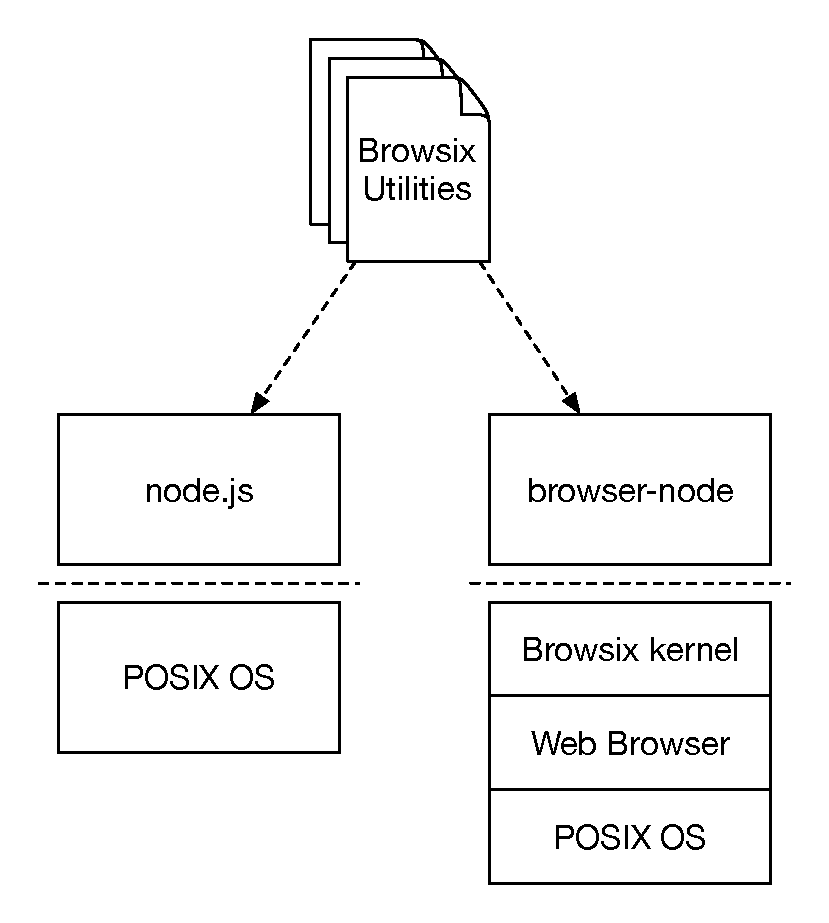
\epsfig{file=img/utilities.eps, height=3in}
\caption{Utilities implemented for Browsix were designed to run in 2
  execution environments - node.js on a traditional OS, as well as in
  a browser through \texttt{browser-node} and the Browsix kernel.}
\end{figure}

To run these utilities in the browser, we developed
\texttt{browser-node} and the Browsix kernel.  This is a port of
node.js to our in-browser process model.  \texttt{browser-node}
utilizes over a dozen of node.js's pure-JavaScript modules directly,
with almost no modification.  Some of these modules, like
\texttt{'internal/util'} are self-contained - they don't depend on any
other modules, or their transitive-dependencies are pure-JavaScript.
However, most modules make foreign function interface (FFI) calls into
node C++ functions and methods.  \texttt{browser-node} provides
pure-JavaScript (written in TypeScript, then compiled) implementations
of these functions and methods.  Our implementations use Web Worker
APIs to post messages representing syscalls to the kernel, invoking
callbacks (back into the node JavaScript libraries) when the kernel
responds in-kind with a syscall-response message.

A consequence of this approach is that only async APIs are
implemented.  No synchronous APIs that require invoking a system call,
such as the methods ending in \emph{Sync} in \texttt{fs}, are
available.

\section{System Design}

The system was designed as 5 major components: a kernel,
\texttt{browser-node}, a shell, UNIX utilities, and a Web Terminal for
the shell.  This approach has led to a system that is straightforward
to extend, and is easy to compare to traditional UNIX programming
environments in terms of behavior.

\subsection{Kernel}

The kernel is modeled after a standard classic UNIX kernel, with some
inspiration taken from Linux.  Its main data members are a single
shared filesystem tree provided by BrowserFS, along with a list of
currently running and recently exited processes.  While BrowserFS
provides a single filesystem root, there maybe several instantiated
filesystems, combined either through the use of an overlay filesystem
or through filesystem mountpoints.

The kernel communicates with process running in Web Workers (referred
to as userspace processes) over a MessagePort provided by the browser.
This has several consequences.  First, messages sent to and from Web
Workers are copied, resulting in a shared-nothing architecture.  This
combined with the way workers are isolated and scheduled means that
the syscall roundtrip path is orders of magnitude more expensive than
on modern operating systems like Linux. There is a mechanism to
transfer ownership of certain types of objects (notably ArrayBuffers),
but this is an optimization that is not used in this project.  Second,
because communication with the worker is based on message passing and
JavaScript has no control over message buffer sizes or the
schedulability of the worker, there is no way to enforce that
processes do not continue to execute while waiting for the results of
a syscall from the kernel without cooperation.  This is a major point
- worker processes are essentially cooperatively scheduled with
respect to the kernel.

There is a small `syscall` layer (module) that lives in the userspace
process.  It is useful to think of that as conceptually part of the
kernel - it is the ABI that the kernel provides to processes;
processes do not need to know anything about message passing, they
simply invoke system calls, providing a callback to receive the result
as the final argument.  The syscall layer also provides a way to
register for delivery of signals, such as \texttt{SIGCHLD}.

\subsubsection{Task Scheduler}

As Web Workers cannot be explicitly preempted by the kernel, the
kernel requires cooperation with processes to ensure fairness.  This
is perhaps not as daunting as it seems - all 17 of our utilities do
not need to know how to cooperate, just the single
\texttt{browser-node} interpreter does.

\subsection{\texttt{browser-node}}

As discussed in the Approach section, browser-node provides an
execution environment for unmodified node.js programs in the browser.
The JavaScript-facing API of node is itself written in JavaScript.

\subsection{Shell}

\subsection{Utilities}

As discussed above, a number of standard UNIX utilities were
implemented from scratch in TypeScript using standard node.js APIs.
Of note was the use of node's Stream objects rather than directly
performing \texttt{read(2)}s and \texttt{write(2)}s on file
descriptors.  This led us to implementations that feel very at home in
the node ecosystem, rather than looking like transliterations of C
programs.  Additional information is given in the Approach section
above.

\subsection{Web Terminal}

The web terminal is implemented using Web Components and the Polymer
library.  This allows us to define a single new tag for use in the
HTML of any application, where a shell can be inserted in 2 lines, by
first doing an HTML import of the \texttt{"browsix-terminal.html"}
file, and then by placing one or multiple
\texttt{"<browsix-terminal>"} tags on the page.  This terminal web
component owns a kernel instance, and invokes methods on the kernel to
evaluate commands and pipelines.

\begin{figure}
\centering
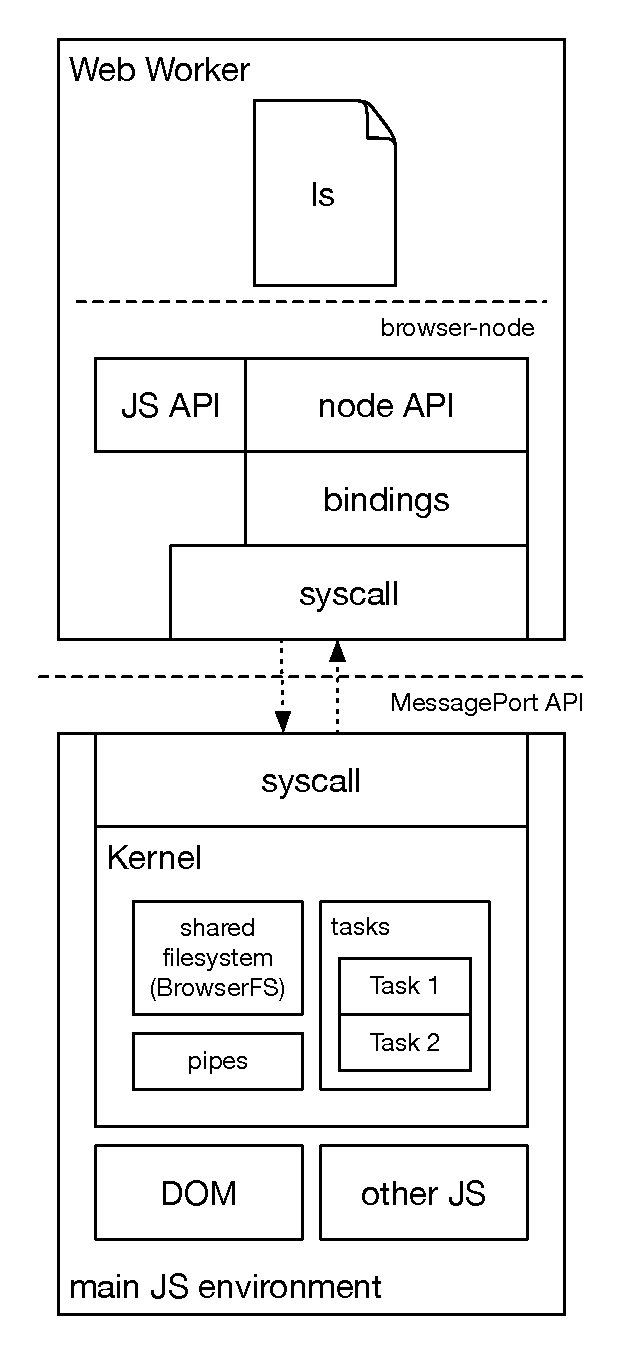
\epsfig{file=img/stack.eps, height=5in}
\caption{The Browsix stack.}
\end{figure}

\section{Results}

The resulting system provides a similar-feeling environment to that of
classic UNIX, BSD, and Plan9 systems, where commands have minimal
options and produce plan-text output.

\section{Discussion}

A downside of the approach taken is that it is somewhat at odds with
the browser's native debug faculties.

\subsection{Further work}

The system call layer that \texttt{browser-node} uses to communicate
with the kernel is not dependent on other parts of
\texttt{browser-node}.  It should be possible to use this layer to
port other runtimes into this process model, such as the Doppio JVM,
emscripten apps built with the emterpreter option, and GopherJS.

\subsubsection{Terminal}

The terminal currently works by taking a line of input, executing it
as a shell, and displaying the results when the command finishes.
This is a fine first step, but interactive UNIX programs (like the
venerable \texttt{ed}) expect that their stdin is hooked up to a
terminal and that writes to stdout appear on the terminal before
program termination.  We don't expect that implementing this
functionality on top of the existing project will require significant
restructuring.

\subsubsection{Pseudo-Filesystems}

Linux and Plan9 before it expose a lot of functionality through the
filesystem, including devices, information on the process tree, and
hardware information.  This is appealing because programs that want to
interact with devices or, for example, the process tree don't need to
learn additional system calls, they just need to read from specific
files and directories.  An interesting area for future work is
providing access to browser APIs to process in Web Workers through
pseudo-filesystems.

\section{Conclusion}

This paper introduced and described the Browsix programming
environment, including the kernel, \texttt{browser-node}, a number of
UNIX utilities implemented in TypeScript, a shell, and web-based
Terminal UI.

\bibliographystyle{abbrv}
\bibliography{report}

\balancecolumns
\end{document}
